\documentclass{standalone}
\usepackage{tikz}
\usetikzlibrary{positioning, shapes.geometric, arrows.meta, calc}

\tikzstyle{startstop} = [rectangle, rounded corners, minimum width=3cm, minimum height=1cm,text centered, draw=black, fill=red!30]
\tikzstyle{io} = [trapezium, trapezium left angle=70, trapezium right angle=110, minimum width=3cm, minimum height=1cm, text centered, draw=black, fill=blue!30]
\tikzstyle{process} = [rectangle, minimum width=3cm, minimum height=1cm, text centered, draw=black, fill=green!30]
\tikzstyle{decision} = [diamond, minimum width=3cm, minimum height=1cm, text centered, draw=black, fill=yellow!30]
\tikzstyle{arrow} = [thick,->,>=Stealth]

\begin{document}
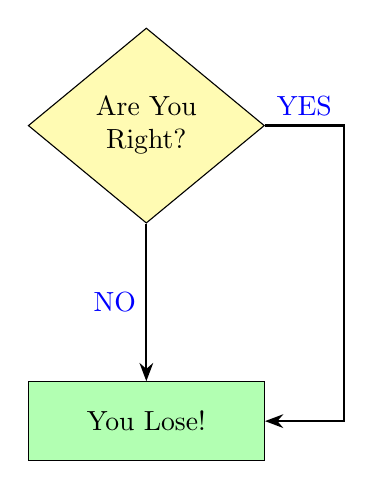
\begin{tikzpicture}[node distance = 2.0cm]
  \node (you) [decision, align = center] {Are You \\ Right?};
  \node (lose) [process, below = of you] {You Lose!};

  \draw[arrow] (you) to node[left, blue]{NO} (lose);
  \draw[arrow] (you.east) to node[above, blue]{YES} ++(1,0) |- (lose.east);
\end{tikzpicture}
\end{document}